\documentclass[UTF8,12pt,a4paper]{ctexart}
\usepackage[a4paper,margin=2.5cm]{geometry}
\usepackage{enumitem}
\usepackage{hyperref}
\usepackage{graphicx}
\usepackage{float}
\usepackage{booktabs}
\usepackage{array}
\usepackage{tabularx}
\usepackage{fancyhdr}
\usepackage{xcolor}
\hypersetup{colorlinks=true,linkcolor=black,urlcolor=blue}
\setmainfont{Times New Roman}
\setCJKmainfont{Songti SC}
\setCJKsansfont{Heiti SC}
\setlength{\parindent}{2em}
\setlength{\parskip}{0.3em}
\setlist[itemize]{leftmargin=2em,itemsep=0.3em,topsep=0.3em}
\renewcommand{\arraystretch}{1.22}
\renewcommand{\thefigure}{3-\arabic{figure}}
\renewcommand{\thetable}{3-\arabic{table}}
\sloppy
\pagestyle{fancy}
\fancyhf{}
\fancyfoot[C]{\thepage}
\renewcommand{\headrulewidth}{0pt}

\begin{document}

\section*{实验3：软件架构与界面设计}

\subsection*{学习通提交说明}

\begin{itemize}
  \item \textbf{提交平台：} 只向学习通对应的“实验报告”作业上传一份PDF文件。
  \item \textbf{文件命名：} 班级-学号-姓名-实验3-软件架构与界面设计.pdf。
  \item \textbf{PDF内容：} 需求与设计对应表、技术选型与架构决策、软件与外部环境关系图、总体架构图与模块说明、数据与接口设计、核心流程图、关键界面原型、设计检查记录及仓库版本证据。
  \item \textbf{截止时间：} 以学习通作业设置为准。
\end{itemize}

\section*{1. 实验目的}

\begin{itemize}
  \item 把实验2的需求说明转化为可指导后续开发的软件架构、模块边界、数据模型、接口和交互方案。
  \item 形成与个人能力匹配的技术选型，并保留关键决策依据。
  \item 完成关键设计，检查需求、架构与界面之间是否一致，为实验4的软件基础功能开发提供设计基线。
\end{itemize}

\section*{2. 实验内容}

\subsection*{2.1 需求输入与设计范围}

\begin{itemize}
  \item 从实验2中选定一条核心用户流程，列出该流程对应的用户故事、功能需求、非功能需求和验收条件，作为本次设计的输入。
  \item 运用软件工程课程中学习的双向追踪原则，先建立“需求编号—准备完成的设计内容—对应图或文档”对应表，确保每项核心需求都有后续设计任务，后续也能从设计内容追溯到需求来源。
  \item 初步划分普通软件功能与AI功能的边界，说明哪些任务可以由确定的程序逻辑完成，哪些任务准备交给LLM处理，以及哪些结果需要程序校验或用户确认。本阶段不要求确定RAG、Agent等具体实现方法。
\end{itemize}

\subsection*{2.2 技术选型与架构决策}

\begin{itemize}
  \item 结合已学习的程序设计语言和软件设计约束，从本人熟悉程度、实现成本、框架生态、AI接入、测试和运行环境等方面比较候选方案。比较可以使用简单表格，不要求罗列过多技术或原因。
  \item 对开发语言与框架、数据保存方式、软件体系结构风格等关键选择编写简短的设计决策说明。设计决策说明也称架构决策记录（ADR），只需写清要解决的问题、考虑过的方案、最终选择、理由和可能的不足。
  \item 为一项可能影响项目继续开发的关键依赖准备替代方案，例如模型服务、数据库或主要框架。
\end{itemize}

\subsection*{2.3 软件架构与模块设计}

\begin{itemize}
  \item 绘制软件与外部环境关系图（也称简化的系统上下文图），标出用户、个人软件、模型或模型服务以及项目需要访问的外部系统或数据源，说明哪些内容属于本软件、哪些属于外部依赖。模型应根据实际运行和调用方式放在合适位置，并注明使用本地模型还是云端模型服务。图形可以参考已经学习的数据流图，用简单的方框和带名称的箭头表示。
  \item 绘制软件总体架构图和模块结构图，根据项目特点选择已学习的分层、MVC等体系结构风格，并可使用包图或构件图表示界面、业务、数据和AI能力等模块。两张图可以合并，但要写明各模块的职责和依赖关系。
  \item 在总体架构图中标明主要数据、调用方向或交互关系，并制作“用户—普通程序—模型—工具职责划分表”，说明核心流程中每一方负责什么以及由谁检查AI结果。
\end{itemize}

\subsection*{2.4 数据、接口与核心流程设计}

\begin{itemize}
  \item 使用已经学习的类图、ER图或其他合适的图形描述核心数据，说明主要数据对象、关键字段、约束和关系，并标明需要保存的数据和敏感数据。
  \item 设计支撑核心用户流程的主要接口，说明接口由哪个模块提供、由谁调用、用途、输入、输出和失败情况，并至少给出一个正常调用与错误调用示例。
  \item 选择已经学习的顺序图、活动图、状态图或普通流程图，描述一次核心任务从用户输入到结果反馈的过程，包含正常路径、失败处理以及必要的人工确认点。
\end{itemize}

\subsection*{2.5 界面原型与交互设计}

\begin{itemize}
  \item 绘制页面结构图、导航关系图或顺序图，说明用户如何从软件入口进入核心功能，以及如何在页面之间跳转、返回、退出或重新操作。
  \item 完成不少于3张关键界面原型图，至少包括首页或入口页、核心任务页和结果页。界面原型是编码前的页面草图，用于确定页面上显示什么以及怎样操作，不要求编写前端代码，可以使用Figma、墨刀、Axure等工具，也可以使用清晰的\textbf{手绘图}。
  \item 结合已经学习的静态元素、动态元素、用户输入元素和用户命令元素，在原型中标注主要信息、输入区域、按钮、输入限制和操作反馈，并补充与项目有关的加载、空数据、错误、重新操作或人工确认状态。
\end{itemize}

\subsection*{2.6 设计一致性检查与版本保存}

\begin{itemize}
  \item 完善2.1建立的需求与设计对应表，补充“架构模块—数据或接口—界面—验收条件”等内容，逐项检查实验2中的核心需求是否已经落实，不需要重新制作一张内容重复的表格。
  \item 记录检查范围、发现的问题和设计调整；如果未发现问题，应说明检查依据。将架构图、数据模型图、流程图、界面原型图和其他设计文件保存到个人GitHub/Gitee仓库并提交。
\end{itemize}

\section*{3. 操作记录}

图必须编号，并配有能够说明图中元素和关系的文字。

\subsection*{3.1 需求与技术选择}

本次围绕“创建课程—设置考试目标—填写掌握度—生成计划—完成任务—更新掌握度—调整计划”进行设计。需求对应情况如下。

\begin{table}[H]
\centering
\caption{需求与设计对应表}
\small
\begin{tabularx}{\textwidth}{p{1.2cm}X X X}
\toprule
编号 & 需求 & 设计内容 & 验收点 \\
\midrule
R1 & 创建课程和考试目标 & 课程、目标模块；首页入口 & 信息可保存和修改 \\
R2 & AI生成学习计划 & AI服务层；计划页 & 结果可编辑、确认 \\
R3 & 完成任务并更新掌握度 & 任务、知识点模块；进度页 & 状态可追踪 \\
R4 & AI失败可继续操作 & 校验与降级流程 & 保留输入，支持手工调整 \\
\bottomrule
\end{tabularx}
\end{table}

技术方案采用Vue负责界面、Python FastAPI负责业务接口、SQLite保存本地数据，并通过可替换的接口调用云端LLM。选择分层结构，便于分别测试界面、业务、AI和数据模块。模型服务不可用时，改用规则模板和手工编辑计划。

\subsection*{3.2 架构与核心流程设计}

系统分为表现层、业务层、AI服务层和数据层。普通程序负责数据保存、日期与字段校验；LLM只生成候选计划；用户负责最终确认。

\begin{figure}[H]
\centering
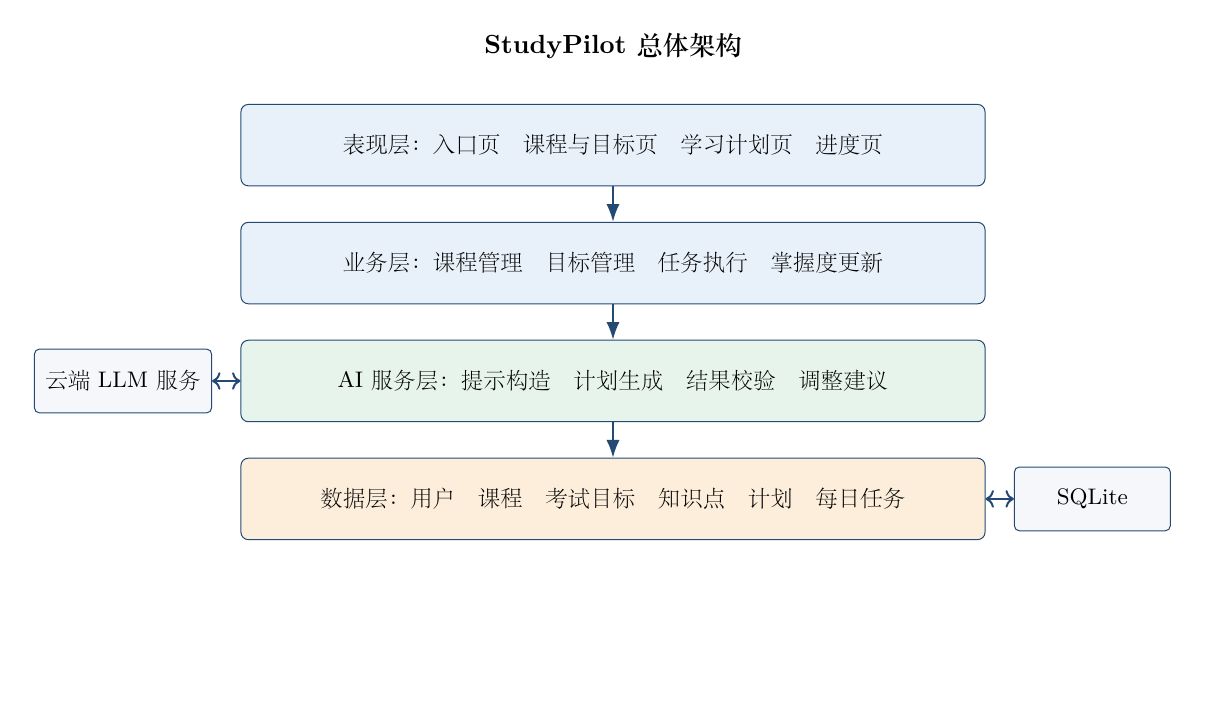
\includegraphics[width=0.94\textwidth]{assets/experiment3/rendered/figure-1.png}
\caption{StudyPilot总体架构图}
\end{figure}

核心流程加入了人工确认点和AI失败后的手工处理入口，避免模型结果直接写入正式计划。

\begin{figure}[H]
\centering
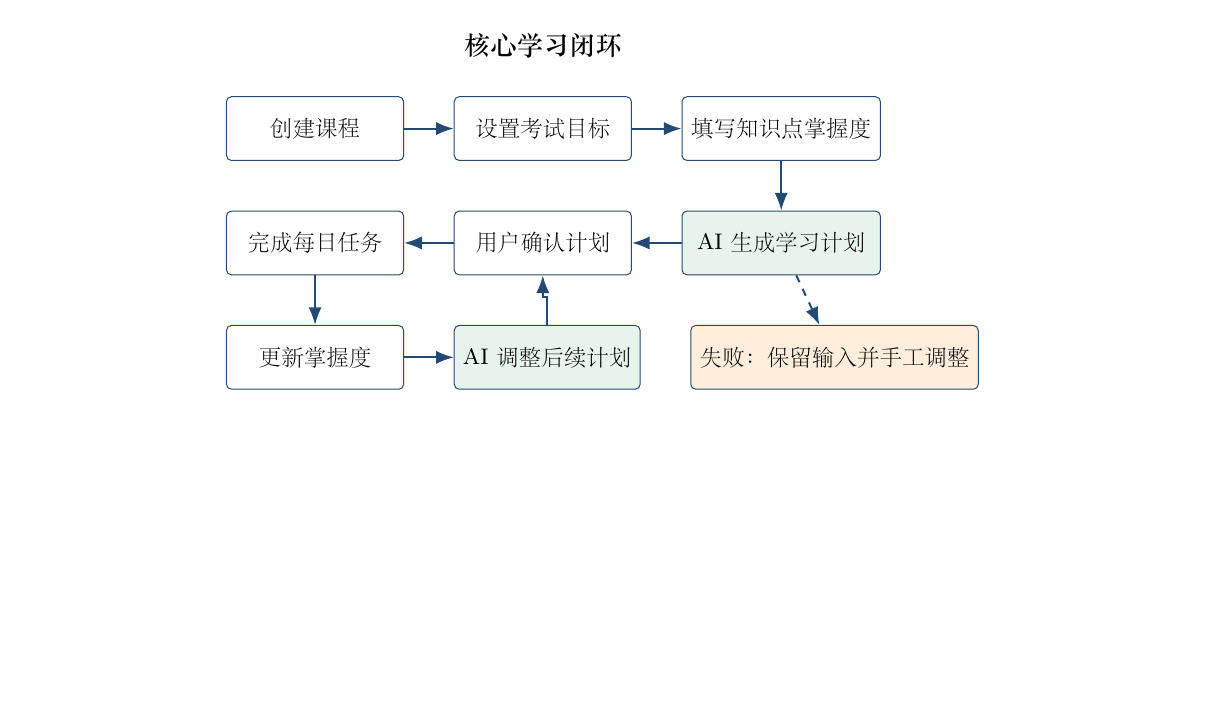
\includegraphics[width=0.92\textwidth]{assets/experiment3/rendered/figure-2.png}
\caption{StudyPilot核心流程图}
\end{figure}

\subsection*{3.3 数据与接口设计}

核心数据包括用户、课程、考试目标、知识点、学习计划和每日任务。掌握度只保存用户输入和确认后的结果，不保存无关个人信息。

\begin{figure}[H]
\centering
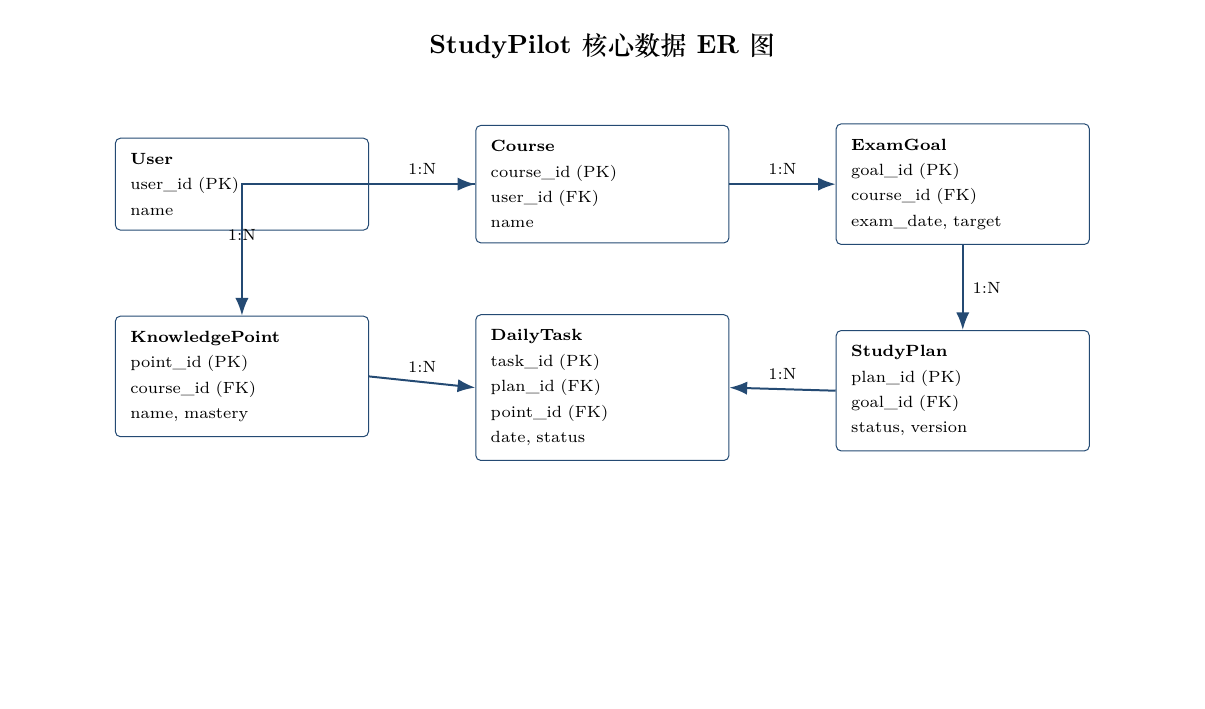
\includegraphics[width=0.94\textwidth]{assets/experiment3/rendered/figure-3.png}
\caption{StudyPilot核心数据ER图}
\end{figure}

主要接口为\texttt{POST /api/plans/generate}。输入课程编号、考试目标、知识点掌握度和可用时间；成功时返回候选任务列表，信息不足时返回错误提示。用户确认后再调用\texttt{POST /api/plans/confirm}保存计划。

\subsection*{3.4 关键界面原型}

首页用于创建课程和进入学习计划；计划页展示AI生成结果并提供确认、重新生成；进度页显示完成情况和掌握度调整建议。

\begin{figure}[H]
\centering
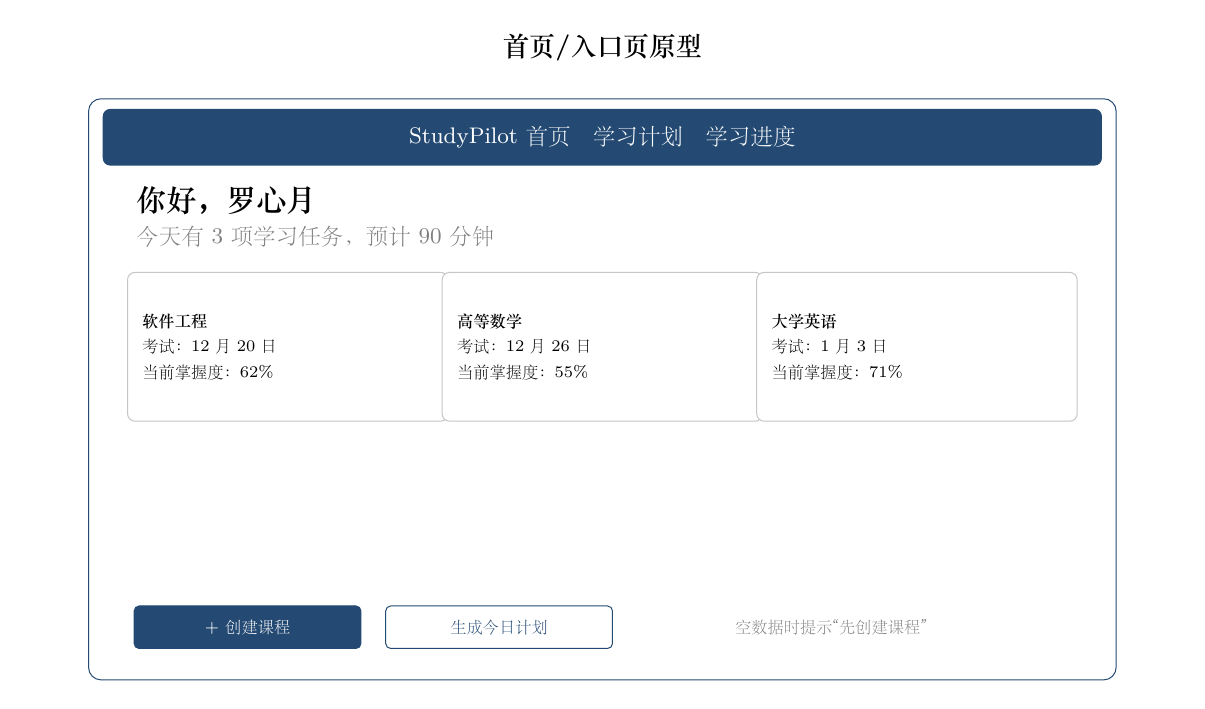
\includegraphics[width=0.92\textwidth]{assets/experiment3/rendered/figure-4.png}
\caption{首页与入口页原型}
\end{figure}

\begin{figure}[H]
\centering
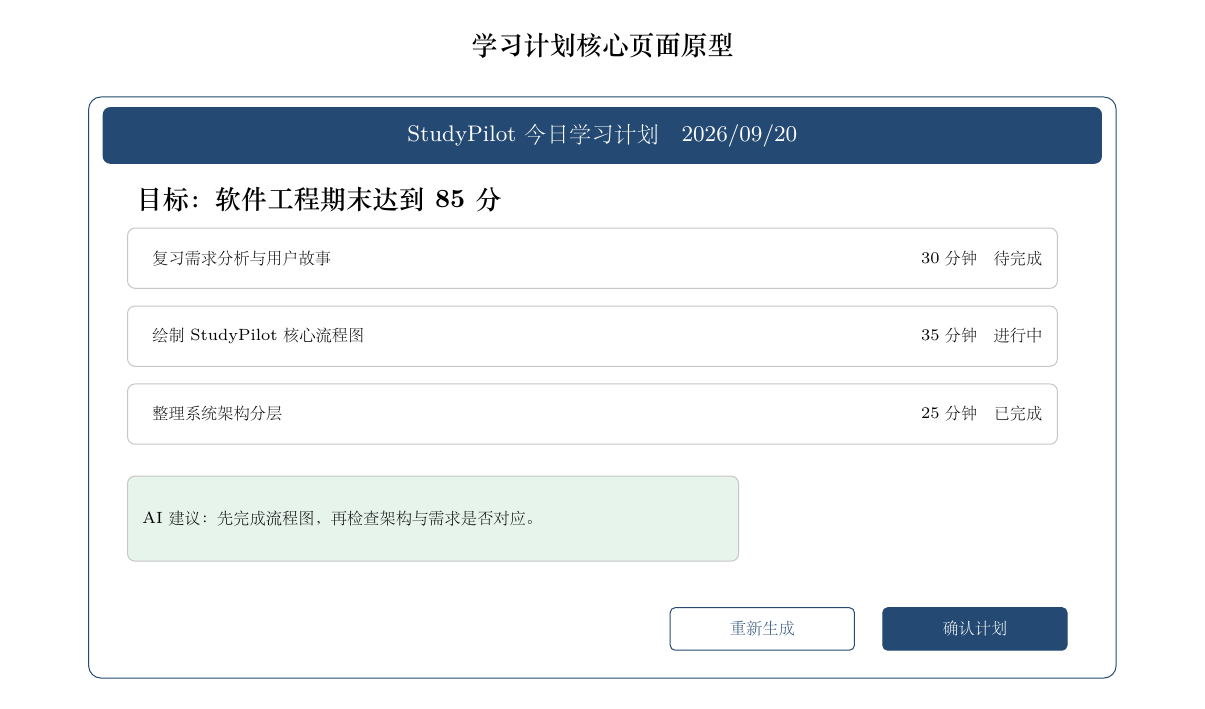
\includegraphics[width=0.92\textwidth]{assets/experiment3/rendered/figure-5.png}
\caption{学习计划核心页面原型}
\end{figure}

\begin{figure}[H]
\centering
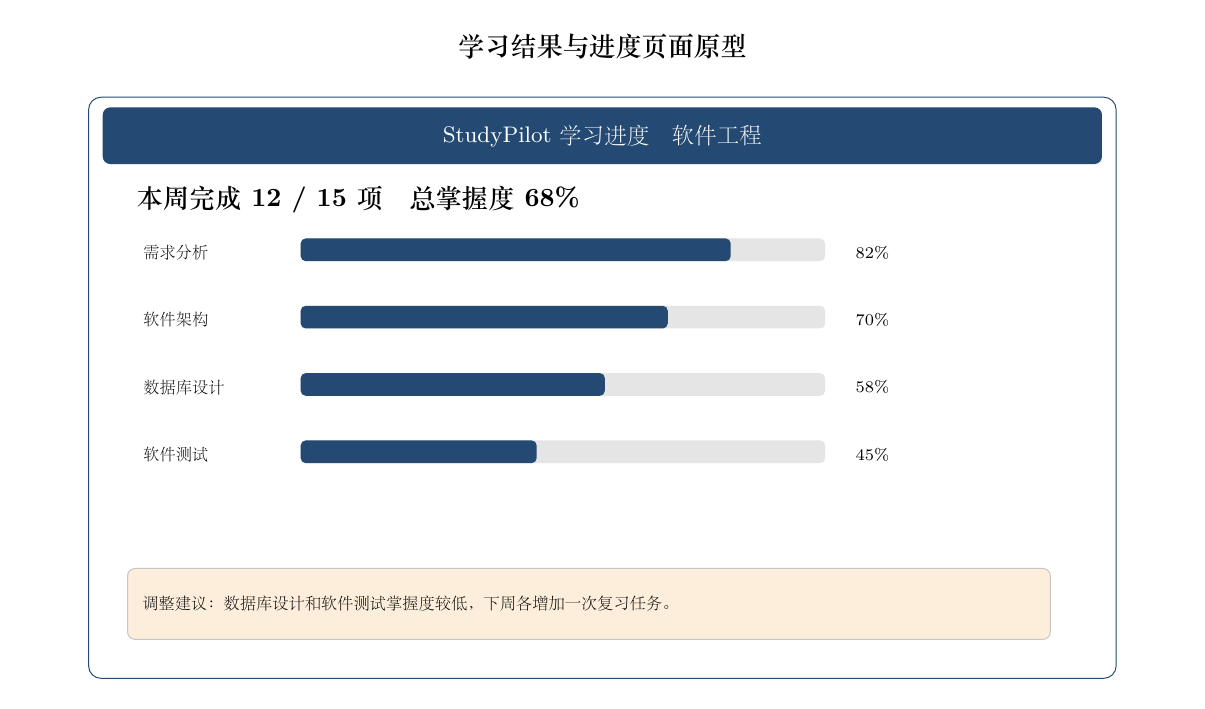
\includegraphics[width=0.92\textwidth]{assets/experiment3/rendered/figure-6.png}
\caption{学习结果与进度页面原型}
\end{figure}

\subsection*{3.5 设计检查与版本记录}

检查时发现两个问题：原流程缺少AI失败处理，已增加手工调整入口；原掌握度准备由系统自动修改，现改为系统建议、用户确认。设计文件已保存到本地Git仓库，提交编号为\texttt{7ecf19a}。

\begin{figure}[H]
\centering
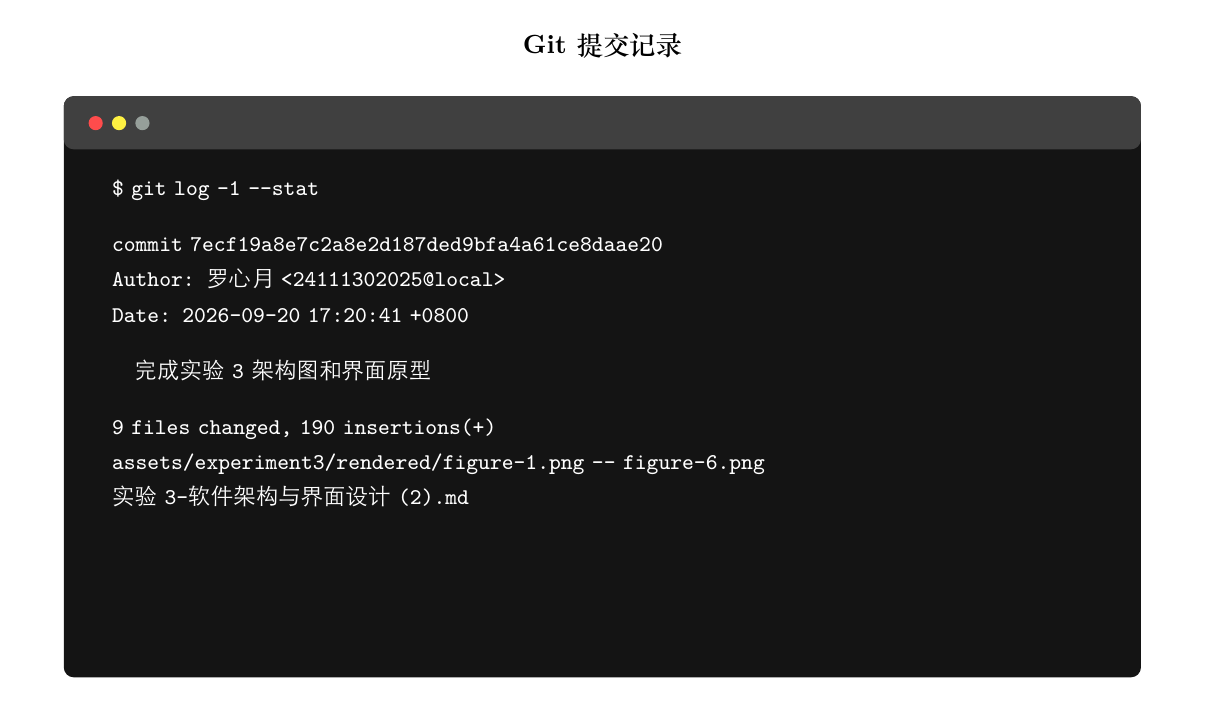
\includegraphics[width=0.92\textwidth]{assets/experiment3/rendered/figure-7.png}
\caption{Git提交记录}
\end{figure}

\section*{4. 实验小结}

本次完成了StudyPilot的分层架构、核心流程、数据关系和三张关键界面原型，设计内容能够支撑后续基础功能开发。设计过程中补充了AI失败后的手工处理入口，并把掌握度自动更新改为用户确认后更新，使流程更稳定，也更符合实际使用情况。

\end{document}
